% Generated by build_paper.py from eon-whitepaper.md.
% Edit Markdown, then regenerate; do not edit this file independently.
\documentclass[11pt,a4paper]{article}
\usepackage{iftex}
\ifPDFTeX
  \usepackage[T1]{fontenc}
  \usepackage[utf8]{inputenc}
\else
  \usepackage{fontspec}
\fi
\usepackage{lmodern}
\usepackage[margin=1in]{geometry}
\usepackage{microtype}
\usepackage{graphicx}
\makeatletter
\define@key{Gin}{alt}{}
\makeatother
\usepackage{float}
\usepackage{placeins}
\usepackage{flafter}
\usepackage[font=small,labelfont=bf,justification=raggedright,singlelinecheck=false]{caption}
\usepackage{booktabs,longtable,array,calc}
\usepackage{listings}
\usepackage{xcolor}
\usepackage{amsmath,amssymb}
\usepackage{enumitem}
\usepackage{titlesec}
\usepackage{fancyhdr}
\usepackage{xurl}
\usepackage[hidelinks]{hyperref}
\definecolor{accent}{HTML}{126B70}
\definecolor{ink}{HTML}{263238}
\definecolor{shade}{HTML}{F1F4F4}
\color{ink}
\pagestyle{fancy}
\fancyhf{}
\fancyhead[L]{\footnotesize Tomorrow's Newspaper}
\fancyhead[R]{\footnotesize\thepage}
\setlength{\headheight}{14pt}
\renewcommand{\headrulewidth}{0.3pt}
\titleformat{\section}{\normalfont\Large\bfseries\color{accent}}{}{0em}{}
\titleformat{\subsection}{\normalfont\large\bfseries}{}{0em}{}
\titlespacing*{\section}{0pt}{2.5ex plus 1ex}{1.4ex}
\titlespacing*{\subsection}{0pt}{2ex plus 1ex}{1ex}
\setcounter{secnumdepth}{-1}
\setcounter{tocdepth}{1}
\setlength{\parindent}{0pt}
\setlength{\parskip}{5pt plus 1pt}
\setlength{\emergencystretch}{3em}
\raggedbottom
\clubpenalty=1000
\widowpenalty=1000
\displaywidowpenalty=1000
\renewcommand{\arraystretch}{1.12}
\renewcommand{\topfraction}{.95}
\renewcommand{\bottomfraction}{.85}
\renewcommand{\textfraction}{.05}
\renewcommand{\floatpagefraction}{.65}
\setlength{\textfloatsep}{14pt plus 2pt minus 2pt}
\setlength{\intextsep}{12pt plus 2pt minus 2pt}
\setlist{nosep,leftmargin=*}
\newcommand{\tightlist}{\setlength{\itemsep}{0pt}\setlength{\parskip}{0pt}}
\newcommand{\passthrough}[1]{#1}
\newcommand{\pandocbounded}[1]{#1}
\lstset{basicstyle=\ttfamily\footnotesize,backgroundcolor=\color{shade},
  frame=none,framesep=6pt,breaklines=true,columns=fullflexible,
  keepspaces=true,showstringspaces=false,breakatwhitespace=false}
\begin{document}
\hypersetup{pageanchor=false}
\begin{titlepage}
\raggedright
\hyphenpenalty=10000
\vspace*{1.5cm}
{\color{accent}\small EREBUS OBSERVATORY NETWORK / EON\par}
\vspace{1cm}
{\Huge\bfseries Tomorrow's Newspaper\par}
\vspace{.8cm}
{\Large Testing a language-model analyst on filings it could not have read\par}
\vspace{1.3cm}
{\large Gabriel George\par}
\vspace{.5cm}
{\large Technical white paper\par}
29 September 2026
\vfill
\noindent\textcolor{accent}{\rule{\textwidth}{1pt}}
\vspace{.5cm}
{\small A language model read 6,653 annual reports. This is how to test it honestly.\par
Research, not investment advice.}
\end{titlepage}
\hypersetup{pageanchor=true}
\pagenumbering{roman}
\tableofcontents
\clearpage
\pagenumbering{arabic}

\section{Abstract}\label{abstract}

EON began in May 2025 as a folder of scripts that read 11,741 annual reports to learn what
excellent companies share. It became a system that reads every 10-K of the listed market
through three fixed lenses and ends each reading in one verdict: 6,653 company-years of 1,358
companies, 500 a day, at the ceiling of a free-tier quota.

An early backtest looked excellent. But most of its outcomes ended before the model's knowledge
cutoff of January 2025, so the model may simply have known how those years ended. \textbf{A
language model's verdicts can only be tested on filings it could not have read.}

On a protocol fixed in advance, the one-year BUY-minus-SELL spread before the cutoff is 13.1
points (p = 0.0001), and about 40\% of it is an industry tilt. After the cutoff, the tilt is
gone; a rank spread of 5.9 percentile points remains (p = 0.0051), on one vintage and a
statistic added late.

The 2025 scripts left something better: scores recorded before their outcomes existed. Tested
now, the headline score, resemblance to 39 excellent companies, pointed the wrong way (Spearman
\ensuremath{-}0.14, p = 0.0001). A contrarian score and options calls showed nothing. The clean tests do not
agree, and that is the finding: a fluent reader is not thereby a forecaster. Fix the model,
date every reading, and keep the ledger.

\emph{This is research, not investment advice.}

\clearpage
\section{1. The question}\label{the-question}

\subsection{1.1 The interaction}\label{the-interaction}

A 10-K is the most complete account a public company gives of itself. It is also long,
repetitive and read closely by few people. I wanted a reader that never tires: one that would
give every filing the same careful attention and leave a record I could count.

EON gives a model one filing and asks one fixed question in three parts. As Warren Buffett
would: is there a durable moat, a capable management, a fair price? As Nassim Taleb would: what
breaks this company, and what would make it stronger under stress? As a contrarian would: what
does the consensus believe, and why might it be wrong? A synthesis weighs the three and ends in
a verdict: STRONG BUY, BUY, HOLD, SELL or STRONG SELL, with a conviction level.

\begin{figure}[!htbp]
\centering
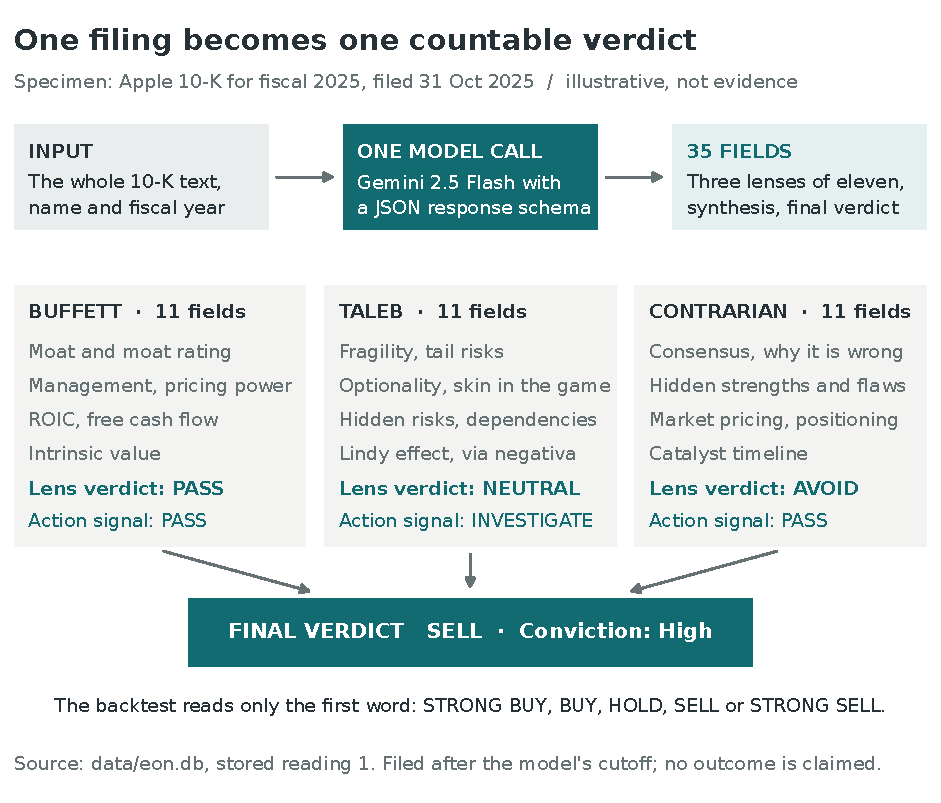
\includegraphics[width=1\linewidth,height=\textheight,keepaspectratio,alt={A 10-K enters one Gemini 2.5 Flash call and leaves as 35 structured fields: three lenses of eleven fields, a synthesis, and a final verdict of SELL with high conviction.}]{figures/01-one-reading.pdf}
\caption{One filing becomes one countable verdict. The specimen is the first stored reading:
Apple's 10-K for fiscal 2025, filed 31 October 2025. The three lens verdicts disagree in
wording; the synthesis resolves them into one. The filing postdates the model's knowledge
cutoff, and no outcome is claimed for it. Illustrative, not evidence. Source:
data/eon.db.}\label{fig:01-one-reading}
\end{figure}

The readings are specific. Apple's Taleb lens finds ``Total Debt/EBITDA ratio of 0.68x in 2025
(\$98,657M debt / \$144,748M EBITDA)'', well below its 3x concern threshold. The final verdict
begins: ``SELL. Conviction: High. Apple is an undeniably excellent company, but a high
conviction SELL rating is warranted given the significant disconnect between its robust
fundamentals and its highly stretched valuation.''

The verdict is what makes a reading countable (Figure 1). The prose around it is for a person;
the first word is for measurement.

\subsection{1.2 The constraints}\label{the-constraints}

{\def\LTcaptype{table} % do not increment counter
\par\addvspace{8pt}\noindent\begin{minipage}{\linewidth}\small
\begin{tabular}{@{}
  >{\raggedright\arraybackslash}p{(\linewidth - 2\tabcolsep) * \real{0.3400}}
  >{\raggedright\arraybackslash}p{(\linewidth - 2\tabcolsep) * \real{0.6600}}@{}}
\toprule\noalign{}
\begin{minipage}[b]{\linewidth}\raggedright\bfseries
Constraint
\end{minipage} & \begin{minipage}[b]{\linewidth}\raggedright\bfseries
Why it binds
\end{minipage} \\
\midrule\noalign{}


Free-tier model quotas & 25 keys at 20 requests a day: 500 readings a day, at most \\
The whole filing, every time & No summaries or excerpts; the model reads what an analyst
would \\
A fixed schema & Readings must be comparable across companies and years \\
Every result survives a restart & A market-wide batch runs for weeks and will be interrupted \\
An evaluation that can fail & A test the model can pass from memory measures nothing \\
\bottomrule\noalign{}
\end{tabular}
\end{minipage}\par\addvspace{8pt}
}

The first and last constraints shape the paper. The quota decided how EON is built. The last
constraint decided how it is judged.

\subsection{1.3 Which evidence belongs to which claim}\label{which-evidence-belongs-to-which-claim}

Several samples appear below. They overlap, so each claim is tagged against this table.

{\def\LTcaptype{table} % do not increment counter
\par\addvspace{8pt}\noindent\begin{minipage}{\linewidth}\small
\begin{tabular}{@{}
  >{\raggedright\arraybackslash}p{(\linewidth - 6\tabcolsep) * \real{0.1900}}
  >{\raggedleft\arraybackslash}p{(\linewidth - 6\tabcolsep) * \real{0.2200}}
  >{\raggedright\arraybackslash}p{(\linewidth - 6\tabcolsep) * \real{0.3500}}
  >{\raggedright\arraybackslash}p{(\linewidth - 6\tabcolsep) * \real{0.2400}}@{}}
\toprule\noalign{}
\begin{minipage}[b]{\linewidth}\raggedright\bfseries
Sample
\end{minipage} & \begin{minipage}[b]{\linewidth}\raggedleft
Size
\end{minipage} & \begin{minipage}[b]{\linewidth}\raggedright\bfseries
What it is
\end{minipage} & \begin{minipage}[b]{\linewidth}\raggedright\bfseries
Used for
\end{minipage} \\
\midrule\noalign{}


\textbf{All readings} & 6,653 & Unique company-years from the three-lens schema, 1,358
companies & Verdict mix (§6) \\
\textbf{February backtest} & 4,689 & Readings available on 12 February 2026, 515 tickers &
Reported results (§7.1) \\
\textbf{Priced readings} & 6,203 & Readings with a parsed verdict, a filing date and prices &
This evaluation (§9) \\
\textbf{Before the cutoff} & 1,099 BUY, 657 SELL & One-year window closed before 31 January
2025 & Historical test (§9.1--9.2) \\
\textbf{After the cutoff} & 339 BUY, 201 SELL & Filed after 31 January 2025, one-year outcome
observed & Clean test (§9.3) \\
\textbf{2025 ledger} & 1,784 / 1,797 / 874 & Compounder, contrarian and options scores from
May--June 2025, with outcomes & Forward test (§9.5) \\
\bottomrule\noalign{}
\end{tabular}
\end{minipage}\par\addvspace{8pt}
}

\section{2. Where it started: a study of excellence}\label{where-it-started-a-study-of-excellence}

Before EON had a name, it was a folder of Python scripts asking a narrower question: what do
excellent companies have in common, and who else has it?

In early May 2025 the scripts downloaded up to thirty years of 10-Ks for 39 long-run
compounders and had Gemini 2.5 Flash, then an April preview, read each one. The readings were
distilled into a meta-analysis of shared success factors, dated 9 May. Between 10 and 13 May
the same scripts read the recent filings of about 1,900 other companies and scored each from 0
to 100 on its resemblance to that pattern. In all: 11,741 filing readings of 2,175 companies,
covering fiscal years 1994 to 2025, as many as 4,641 in a single day.

Two more passes followed. On 26 May a contrarian scan scored 1,933 companies on six ``alpha''
dimensions. On 4 June an options pass read the same companies again and made 951 directional
calls: buy calls or buy puts.

Almost everything in EON descends from these weeks: reading whole filings, the contrarian
scanner's six dimensions, the options workflows, and the corpus of excellent-company factors
that the Moonshot \ensuremath{\times} Excellence screener still loads.

So do two of its lessons. The outputs had no fixed schema. The script that later flattened them
found the six success factors spelled about 130 different ways. And the model did not know what
day it was. Run in May 2025, it stamped 1,916 of its 1,919 comparative analyses with a date in
2024, and 91 of the options readings suggested expiries in 2024, already in the past.

The 2025 outputs were saved and never changed. That turned out to be their most valuable
property: they are a ledger written before its outcomes (§9.5).

\section{3. Design one: a workflow builder}\label{design-one-a-workflow-builder}

The project, then called Fintel, returned in December 2025 as an application. Its centrepiece
was a visual workflow builder. A user chained steps (choose companies, fetch filings, run an
analysis, filter, aggregate, export) and ran the chain. The archive holds 16 saved workflows
and 26 workflow runs from 7 to 30 December 2025, among 250 analysis runs by mid-January.

It was the right way to learn which questions were worth asking. The saved chains compare three
chip makers, read three nuclear start-ups through one lens, and pull executive pay from a proxy
statement.

It was the wrong way to learn whether any answer was right. Each chain asked its own question
of its own companies. No two runs were comparable, and nothing accumulated. A pile of good
essays is not a dataset.

The builder was removed on 30 December 2025. What it taught stayed: the three lenses, the
structured output, and the idea, first glimpsed in May, that the question should be written
once and asked of everything.

\section{4. Design two: one question, every filing}\label{design-two-one-question-every-filing}

\subsection{4.1 The schema is the instrument}\label{the-schema-is-the-instrument}

Design two fixes the question. One prompt, one response schema, and every listed company's
recent 10-Ks. The schema has 35 fields: eleven for each lens, a synthesis, and the final
verdict. Pydantic validates every response; a reading that does not fit the schema is not
stored.

Fixing the question turns a model's opinions into a panel: the same measurement, taken on 1,358
companies over six fiscal years. That is what makes everything later in this paper possible.

\begin{quote}
A fixed question asked of every filing turns a language model from a conversation into an
instrument.
\end{quote}

\subsection{4.2 The quota is the clock}\label{the-quota-is-the-clock}

Every reading is one request, and requests are rationed. EON rotates 25 API keys, each allowed
20 requests a day, with file locks so that parallel workers, the command line and the web
interface never spend the same request twice.

The market-wide batch ran from 8 to 21 February 2026. It read 6,568 filings from 1,327
companies. Figure 2 shows its rhythm: a burst after the quota reset at midnight Pacific, then
silence until the next.

\begin{figure}[!htbp]
\centering
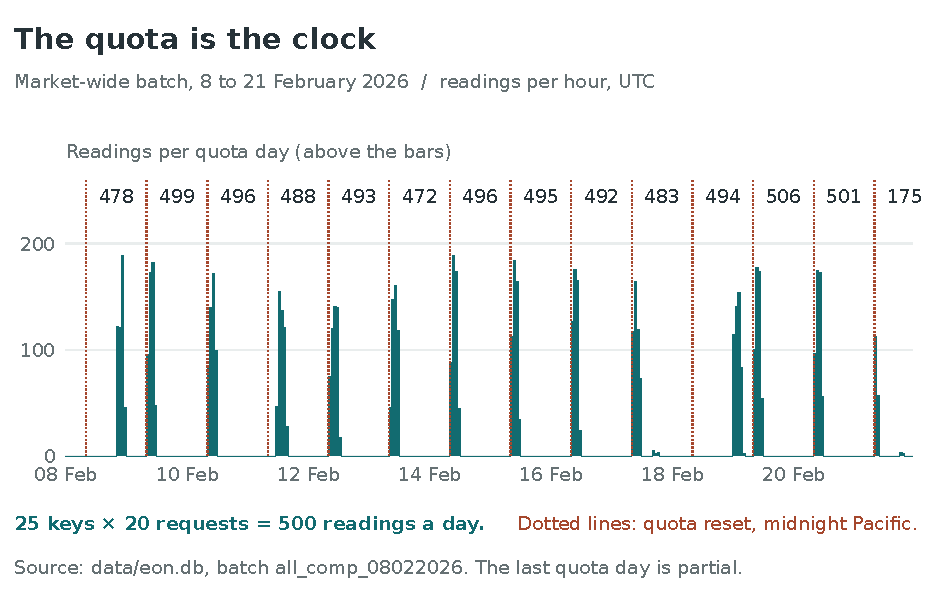
\includegraphics[width=1\linewidth,height=\textheight,keepaspectratio,alt={Hourly readings over 14 days show a burst after each 08:00 UTC quota reset and near silence in between, with 472 to 506 readings in every full quota day.}]{figures/02-quota-clock.pdf}
\caption{The quota is the clock. Every full quota day read between 472 and 506 filings, against
a ceiling of 500; the day boundary here is approximate, so a day can exceed it slightly. The
last day is partial. Hours are UTC; the reset is midnight Pacific, 08:00 UTC in February.
Source: data/eon.db, batch all\_comp\_08022026.}\label{fig:02-quota-clock}
\end{figure}

A clock this slow changes what engineering matters. A 1,000-company, ten-year batch is 20 days
of quota. So EON saves each fiscal year's result the moment it arrives, holds a lease on each
company with a heartbeat, and resumes an interrupted company from its last completed year. When
every key is spent, it waits for the reset and continues. None of this is novel. It is what a
rationed reader needs.

\subsection{4.3 What happens to a filing}\label{what-happens-to-a-filing}

EON downloads each 10-K's HTML from SEC EDGAR, renders it to PDF in headless Chrome, extracts
the text with PyPDF2, and appends all of it to the prompt. No filing is truncated. A filing too
long for the model's context is marked skipped, not cut.

The route through PDF is a detour, and it costs a browser process per filing. It does not
affect the evaluation, but a cleaner pipeline would parse the HTML directly.

Of the 1,410 companies in the market-wide batch, 83 failed: 61 because no 10-K could be
retrieved, and 22 because the model call failed after retries.

\section{5. Design three: workflows as hypotheses}\label{design-three-workflows-as-hypotheses}

With the panel built, I began writing narrower questions as custom workflows: auto-discovered
Python files, each with its own prompt and schema. Two lessons from this period shaped the
tools, and one of them reappears in the results.

\textbf{Schema size is a reliability budget.} The CSPP workflow first asked for a whole
analytical framework in one call. Its schema was about 106 KB, 28 times the size of one lens.
When any of its roughly 200 required fields drifted, validation failed and the whole reading
was lost. On 20 May 2026 it was split into four calls of lens-sized schemas, merged afterwards,
with a partial result kept if one call fails.

\textbf{Let the model judge; let code count.} The same rewrite stopped trusting the model's
arithmetic: domain totals and the master score are recomputed in Python from the model's
component scores. The Moonshot \ensuremath{\times} Excellence screener of 4 June 2026 goes further. The model
rates six dimensions on anchored 0 to 10 scales, each defined at 0, 5 and 10, and code computes
the weighted totals.

That screener also shows the quota as a design constraint. It deliberately uses one call rather
than two. It injects a reference corpus of up to 250,000 tokens, and a second call would resend
it and spend a second request per company.

\begin{figure}[!htbp]
\centering
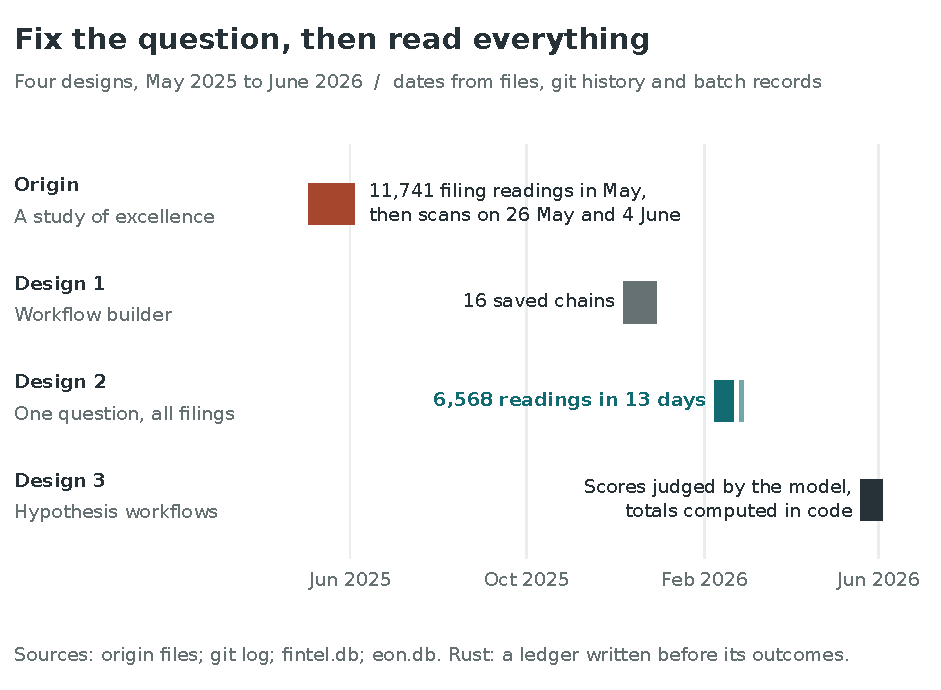
\includegraphics[width=1\linewidth,height=\textheight,keepaspectratio,alt={A timeline from December 2025 to June 2026 shows the workflow builder in December, the market-wide batch in February, and hypothesis workflows in May and June.}]{figures/03-three-designs.pdf}
\caption{Four designs, one idea: fix the question, then read everything. The origin's dates
come from its output files, later dates from git history and stored readings. The rust bar
marks the 2025 readings, recorded before any of their outcomes existed. Bar length is calendar
time, not effort. Sources: the origin project; git log; data/archive/fintel.db;
data/eon.db.}\label{fig:03-three-designs}
\end{figure}

Each design kept what the last one taught (Figure 3). The project has run for seventeen months.
None of its designs, by itself, said whether the readings were right.

\section{6. What 6,653 readings said}\label{what-6653-readings-said}

Before asking whether the verdicts were right, it is worth seeing what they were. Across 6,411
dated readings, 50.8\% say HOLD, 27.5\% BUY, 16.5\% SELL, 3.8\% STRONG BUY and 1.4\% STRONG
SELL. Conviction is Medium in 4,632 readings, High in 1,516 and Low in 148.

\begin{figure}[!htbp]
\centering
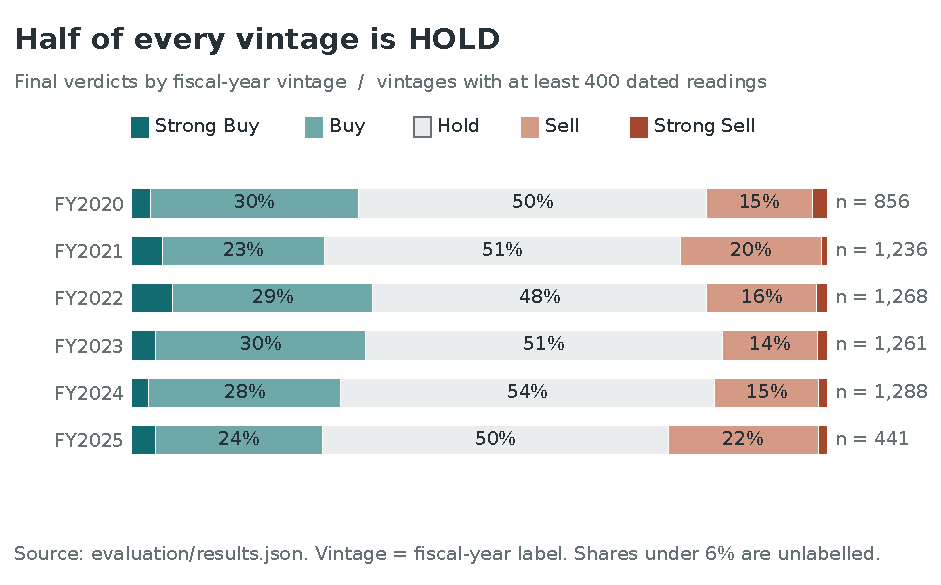
\includegraphics[width=1\linewidth,height=\textheight,keepaspectratio,alt={Stacked bars for fiscal years 2020 to 2025 show HOLD at roughly half of every vintage, BUY near a quarter to a third, and SELL between 15 and 23 percent.}]{figures/04-verdict-mix.pdf}
\caption{Half of every vintage is HOLD: between 48.0\% and 53.6\% in each fiscal year from 2020
to 2025. SELL and STRONG SELL together range from 15.1\% to 22.9\%. Vintage is the fiscal-year
label EON received from EDGAR metadata. FY2025 is partly covered. Source:
evaluation/results.json.}\label{fig:04-verdict-mix}
\end{figure}

The mix barely moves from year to year (Figure 4), across a speculative boom, a bear market and
a recovery. The model is not reading the market's mood into its verdicts, or at least not in
its overall proportions. Whether it reads anything useful about individual companies is the
next question.

\FloatBarrier
\section{7. The February backtest, and the problem of memory}\label{the-february-backtest-and-the-problem-of-memory}

\subsection{7.1 What it reported}\label{what-it-reported}

On 12 February 2026, while the market-wide batch was still running, I ran a backtester over the
readings stored so far. It used 4,689 readings of 515 tickers, entered each position on 1 April
after the fiscal year, and compared returns with SPY. Its report found that BUY-rated stocks
beat SELL-rated ones by 7.1 points over one year (p = 0.003) and 14.1 points over two (p =
0.0008). The two-year result survived clustering by ticker (p = 0.041). High-conviction calls
appeared stronger again: 25.5 points over two years. It concluded that the model showed
``genuine stock selection skill''.

These are reported results from
\passthrough{\lstinline!experimental/backtester/BACKTEST\_REPORT.md!}, not new measurements.

\subsection{7.2 The model has read the answers}\label{the-model-has-read-the-answers}

The report tested every reading against an outcome that had already happened. Gemini 2.5 Flash
has a published knowledge cutoff of January 2025. A reading of a fiscal 2021 10-K, entered in
spring 2022 and judged in spring 2023, asks the model about a period its training data may
describe in detail.

The filing text does not reveal the future. But the prompt names the company and asks for the
consensus view, the market's positioning and the catalysts ahead. The verdicts also weigh
valuation, and a 10-K states no current share price, only the value of the public float some
months before. The model supplies the rest from what it knows. Answering those well invites the
model to draw on everything it knows about the company, and it cannot separate what it knew in
2022 from what it learned later.

\begin{quote}
If a model's training data overlaps the outcome period, a backtest measures its memory as well
as its judgement, and cannot say how much of each.
\end{quote}

Figure 5 shows how much of the history sits on the wrong side of that line.

\begin{figure}[!htbp]
\centering
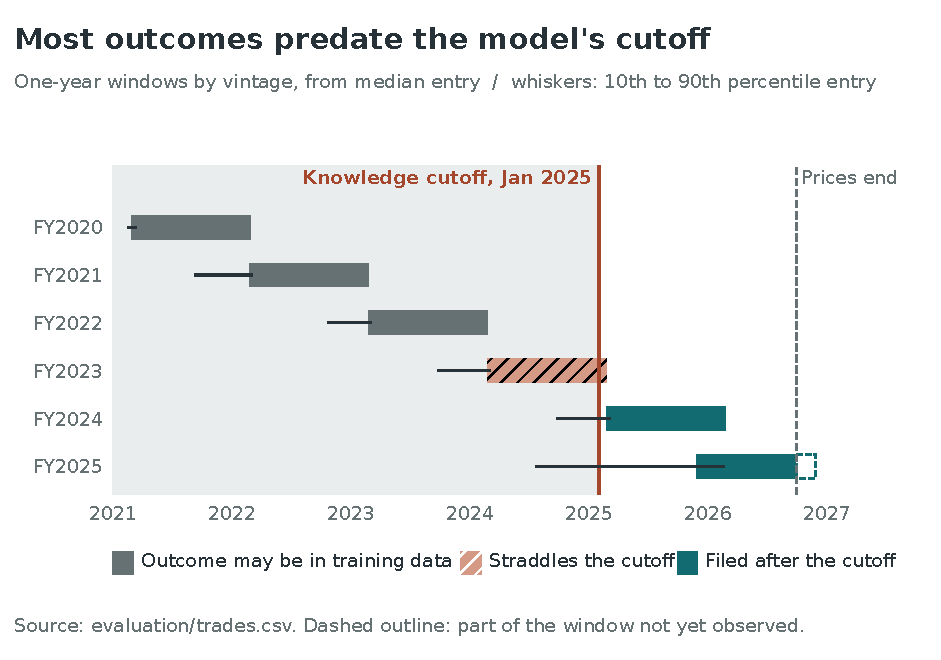
\includegraphics[width=1\linewidth,height=\textheight,keepaspectratio,alt={One-year holding windows for fiscal years 2020 to 2022 end before the January 2025 cutoff, fiscal 2023 straddles it, and fiscal 2024 and 2025 begin after it.}]{figures/05-cutoff-timeline.pdf}
\caption{Most outcomes predate the model's cutoff. Bars are one-year windows from each
vintage's median entry date; whiskers span the 10th to 90th percentile of entries. FY2025's
early entries come from companies whose fiscal-year labels run ahead of the calendar; the
evaluation classifies every reading by its actual filing date. Cutoff: Google's Gemini 2.5
Flash model documentation, ``January 2025''. Source:
evaluation/trades.csv.}\label{fig:05-cutoff-timeline}
\end{figure}

\subsection{7.3 Three smaller problems}\label{three-smaller-problems}

\textbf{Readings are not independent.} A company appears in up to six vintages, and all
readings in a vintage share one market. A t-test over trades treats 1,700 correlated bets as
1,700 independent ones. Clustering by ticker helps with the first problem, not the second.

\textbf{The universe survived.} The companies were listed in February 2026. Firms that failed
or were acquired before then were never read, and 45 tickers that were taken private or
acquired by September 2026 have no prices in the refresh.

\textbf{Entry dates were a convention.} The 1 April entry was never early: 6,386 of 6,411 dated
readings were filed on or before it. It was often late, by up to a year for non-December fiscal
years. Actual filing dates are better.

None of these is as serious as memory. All of them are fixable.

\section{8. A test built around the cutoff}\label{a-test-built-around-the-cutoff}

I wrote the protocol in \passthrough{\lstinline!evaluation-config.yaml!} before the first run.
It fixes five choices.

\begin{enumerate}
\def\labelenumi{\arabic{enumi}.}
\tightlist
\item
  \textbf{One reading per company-year}, the first stored. Overlapping batches had saved some
  twice.
\item
  \textbf{Entry on the first trading day after the actual filing date.} Excess return is the
  stock's return minus SPY's over the same window, at six months, one year and two years (126,
  252 and 504 trading days).
\item
  \textbf{Long means BUY or STRONG BUY; short means SELL or STRONG SELL.} The statistic is the
  difference in mean excess return between them, the spread.
\item
  \textbf{Permutation tests, not t-tests.} Verdicts are shuffled 10,000 times within each
  vintage, and separately within each vintage-and-industry block. The null hypothesis is that a
  verdict carries no information beyond its vintage, or its vintage and industry. This respects
  the shared market of each vintage, which a trade-level t-test ignores.
\item
  \textbf{Two primary questions.} Does the one-year spread survive for windows that closed
  before the cutoff? Does a six-month spread appear for filings published after it?
\end{enumerate}

The first run used the price cache EON already had, which ended on 6 February 2026. It showed
that the historical effect lives at one year and beyond, where the clean sample had no outcomes
yet. Prices through 28 September 2026 made the one-year clean test possible. I made three
amendments, recorded in the config with their reasons:

{\def\LTcaptype{table} % do not increment counter
\par\addvspace{8pt}\noindent\begin{minipage}{\linewidth}\small
\begin{tabular}{@{}
  >{\raggedright\arraybackslash}p{(\linewidth - 4\tabcolsep) * \real{0.3600}}
  >{\raggedright\arraybackslash}p{(\linewidth - 4\tabcolsep) * \real{0.4000}}
  >{\raggedright\arraybackslash}p{(\linewidth - 4\tabcolsep) * \real{0.2400}}@{}}
\toprule\noalign{}
\begin{minipage}[b]{\linewidth}\raggedright\bfseries
Amendment
\end{minipage} & \begin{minipage}[b]{\linewidth}\raggedright\bfseries
Why
\end{minipage} & \begin{minipage}[b]{\linewidth}\raggedright\bfseries
Free parameters
\end{minipage} \\
\midrule\noalign{}


One-year test after the cutoff & Mirrors the historical test exactly & None \\
Rank statistic for every primary sample & One stock moved a mean by \textasciitilde10 points
(§9.3) & None; same blocks \\
Anachronism probe & A direct look for leaked knowledge (§9.4) & Term list and dates \\
\bottomrule\noalign{}
\end{tabular}
\end{minipage}\par\addvspace{8pt}
}

Two parsing corrections followed: verdicts prefixed ``Overall investment recommendation:'', and
conviction written several ways. They added 328 readings and changed no conclusion. The first
run's outputs are kept in \passthrough{\lstinline!evaluation/v1-feb-cache/!}.

\section{9. Results}\label{results}

\subsection{9.1 Before the cutoff: large, and growing with time}\label{before-the-cutoff-large-and-growing-with-time}

For windows that closed before 31 January 2025, BUY-rated filings beat SELL-rated ones by 13.1
percentage points at one year: 1,099 BUY readings at +2.2 points over SPY against 657 SELL
readings at \ensuremath{-}10.9. No permutation within vintage, or within vintage and industry, produced a
spread as large (p = 0.0001 in both, the smallest value 10,000 permutations can give).

The spread grows with the horizon: 3.2 points at six months, 13.1 at one year, 31.6 at two
(Figure 6, grey). At one year the short leg carries most of it. At two years both legs
contribute: +17.0 for BUY, \ensuremath{-}14.6 for SELL.

\begin{figure}[!htbp]
\centering
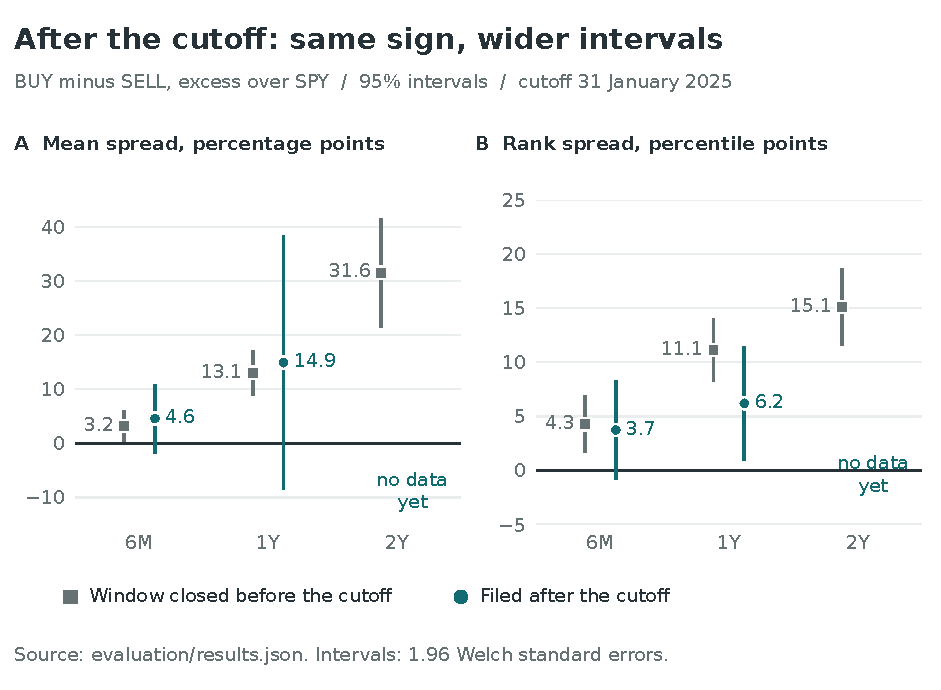
\includegraphics[width=1\linewidth,height=\textheight,keepaspectratio,alt={Two panels plot mean and rank spreads at six months, one year and two years; before the cutoff both rise with horizon; after it, estimates are positive with much wider intervals.}]{figures/06-horizons.pdf}
\caption{After the cutoff: same sign, wider intervals. Grey squares: windows that closed before
31 January 2025. Teal circles: filings published after it. Intervals are 1.96 Welch standard
errors, shown for comparison; the tests in the text are permutation tests. Rank spread is the
difference in mean within-vintage percentile rank. Two-year outcomes do not yet exist after the
cutoff. Source: evaluation/results.json.}\label{fig:06-horizons}
\end{figure}

The sign holds in every vintage, not just on average:

{\def\LTcaptype{table} % do not increment counter
\par\addvspace{8pt}\noindent\begin{minipage}{\linewidth}\small
\begin{tabular}{@{}
  >{\raggedright\arraybackslash}p{(\linewidth - 8\tabcolsep) * \real{0.1400}}
  >{\raggedleft\arraybackslash}p{(\linewidth - 8\tabcolsep) * \real{0.2400}}
  >{\raggedleft\arraybackslash}p{(\linewidth - 8\tabcolsep) * \real{0.1800}}
  >{\raggedleft\arraybackslash}p{(\linewidth - 8\tabcolsep) * \real{0.1800}}
  >{\raggedright\arraybackslash}p{(\linewidth - 8\tabcolsep) * \real{0.2600}}@{}}
\toprule\noalign{}
\begin{minipage}[b]{\linewidth}\raggedright\bfseries
Vintage
\end{minipage} & \begin{minipage}[b]{\linewidth}\raggedleft
BUY / SELL readings
\end{minipage} & \begin{minipage}[b]{\linewidth}\raggedleft
1Y mean spread
\end{minipage} & \begin{minipage}[b]{\linewidth}\raggedleft
1Y rank spread
\end{minipage} & \begin{minipage}[b]{\linewidth}\raggedright\bfseries
Window
\end{minipage} \\
\midrule\noalign{}


FY2020 & 268 / 144 & +18.0 & +14.9 & Before cutoff \\
FY2021 & 331 / 253 & +11.7 & +8.8 & Before cutoff \\
FY2022 & 415 / 212 & +16.4 & +12.1 & Before cutoff \\
FY2023 & 407 / 182 & +8.0 & +7.0 & Straddles \\
FY2024 & 372 / 203 & +9.6 & +5.3 & Mostly after \\
\bottomrule\noalign{}
\end{tabular}
\end{minipage}\par\addvspace{8pt}
}

Spreads are in percentage and percentile points; vintages are fiscal-year labels, so a few
FY2024 filings predate the cutoff. The spread is largest for the vintages entered in early 2021
and early 2023. On the rank measure it is less than half as large for the two most recent.

Taken alone, this would support the February report. It is also exactly what memory would
produce.

\subsection{9.2 Where the historical spread comes from}\label{where-the-historical-spread-comes-from}

The within-industry permutation test separates two things. The mean of its null distribution is
the spread you would expect from the industries the model favoured, with verdicts otherwise
random. The remainder is selection among companies in the same industry.

On the rank statistic, the one-year historical spread of 11.5 percentile points splits into 4.8
points of industry tilt and 6.6 within industry (Figure 7; parts are rounded separately). About
40\% of the historical effect is a bet on industries, and the industries it favoured went on to
do well.

\begin{figure}[!htbp]
\centering
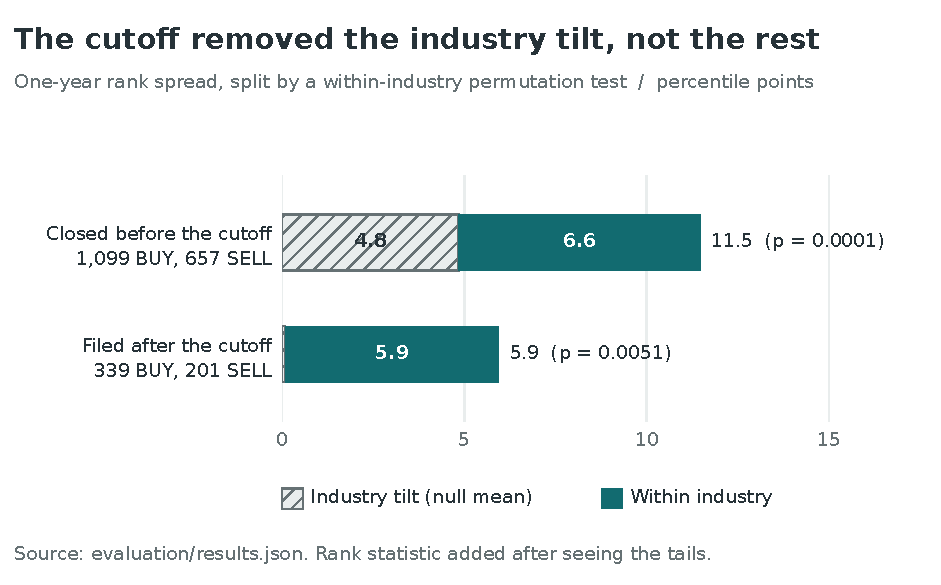
\includegraphics[width=1\linewidth,height=\textheight,keepaspectratio,alt={Stacked bars split the one-year rank spread: before the cutoff 4.8 industry tilt plus 6.6 within industry; after it 0.1 tilt plus 5.9 within industry.}]{figures/07-decomposition.pdf}
\caption{The cutoff removed the industry tilt, not the rest. Industry tilt is the mean of the
within-industry permutation null; the remainder is the within-industry spread. Totals (11.5 and
5.9) differ slightly from Figure 6 (11.1 and 6.2) because the permutation test drops readings
alone in their industry block. Industries are a February 2026 FactSet snapshot. The rank
statistic was added after inspecting the tails (§8). Source:
evaluation/results.json.}\label{fig:07-decomposition}
\end{figure}

\subsection{9.3 After the cutoff: smaller, noisier, not zero}\label{after-the-cutoff-smaller-noisier-not-zero}

After the cutoff there are 1,443 filings, published between 3 February 2025 and 17 March 2026.
Most are fiscal 2024 10-Ks filed in February and March 2025. The model could not have read any
of them in training. The readings were made in February 2026 with web search switched off, so
the filing itself was the model's only source of anything after January 2025.

\textbf{At six months} (the pre-registered clean test), 416 BUY and 275 SELL readings give a
spread of 4.6 points. The within-vintage permutation gives p = 0.11; the within-industry test
gives p = 0.048. The test could only have reliably detected a spread of about 7 points, and the
historical six-month spread was 3.2. It neither confirms nor refutes the historical result.

\textbf{At one year}, 339 BUY and 201 SELL readings give a mean spread of 14.9 points, almost
exactly the historical 13.1. The interval is ±23 points and the permutation p-values are 0.22
and 0.29. The reason is in Figure 8.

\begin{figure}[!htbp]
\centering
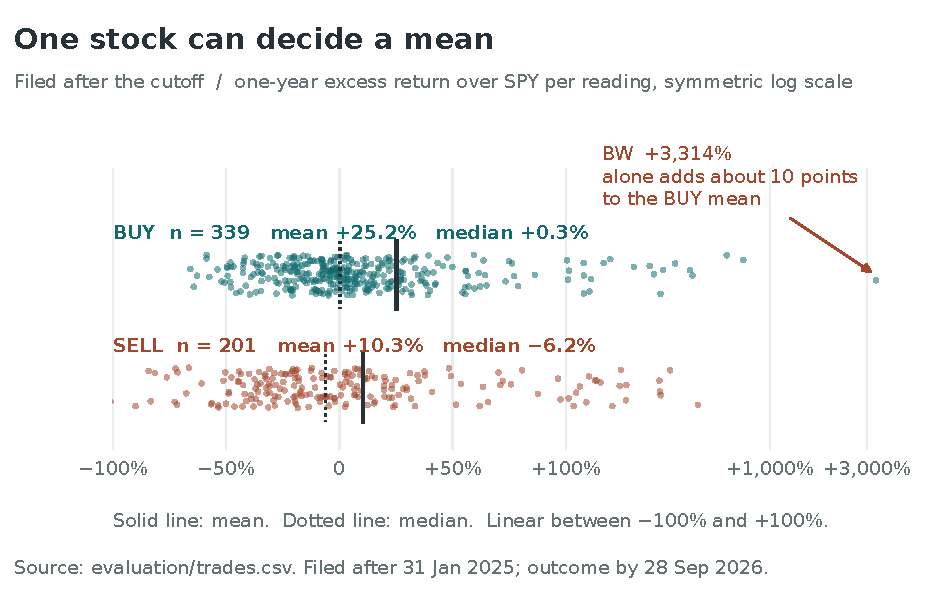
\includegraphics[width=1\linewidth,height=\textheight,keepaspectratio,alt={A strip plot of one-year excess returns after the cutoff shows most readings between \ensuremath{-}60\% and +100\%, with one BUY-rated stock at +3,314\% pulling the BUY mean far above its median.}]{figures/08-tails.pdf}
\caption{One stock can decide a mean. BW's 10-K of 31 March 2025 was read as BUY; the stock
returned 3,314\% more than SPY over the following year, adding about 10 points to the BUY mean
on its own. BUY's mean is +25.2\% and its median +0.3\%. Returns are Yahoo Finance adjusted
closes; BW's has not been checked against a second source. Source:
evaluation/trades.csv.}\label{fig:08-tails}
\end{figure}

A statistic one company can decide cannot answer the question. The rank spread, added for this
reason and applied to every sample alike, gives 5.9 percentile points (p = 0.0051), with a
detectable size of 6.0. Almost none of it is industry tilt: 0.1 points, against 4.8 before the
cutoff. The within-industry part is 5.9, against 6.6 before (Figure 7).

\subsection{9.4 A direct look for leaked knowledge}\label{a-direct-look-for-leaked-knowledge}

If the model's later knowledge leaked into its readings, it might occasionally say so. I
searched every reading for terms that entered public use on known dates, and counted those
appearing in readings of filings published earlier.

The probe has power for one term. The Inflation Reduction Act appears in 300 readings, and in
none of the 2,124 priced readings of filings published before it was signed on 16 August 2022.
The other terms are too rare to test anything: the CHIPS and Science Act appears 12 times, the
rest at most twice. None appears early.

This rules out careless leakage, where the model writes about events the filing could not
contain. It cannot rule out quiet leakage: a verdict nudged by what the model knows, with
nothing in the prose to show it.

\subsection{9.5 A ledger written in 2025}\label{a-ledger-written-in-2025}

Everything above depends on an argument about what the model could have known. The 2025 scores
need no such argument. They were recorded in May and June 2025, after the model's cutoff and
before any of the returns they might predict, and left untouched since.

I tested them under a protocol written before the test, with the same rules as the main
evaluation: entry on the first trading day after each reading, excess return over SPY for one
year (six months for the options calls, their own timeframe), permutations within industry. One
earlier look must be disclosed: on 14 July 2026 I checked the compounder score against raw
returns and found the top fifth had returned 10.4\% against 35.6\% for the bottom fifth.

The protocol confirms it. Across 1,766 companies, resemblance to the 39 excellent companies
predicted \emph{under}performance: Spearman \ensuremath{-}0.14 (p = 0.0001). The top fifth trailed SPY by
17.8 points on average and the bottom fifth beat it by 18.6; the medians, \ensuremath{-}26.5 and \ensuremath{-}11.0, tell
the same story. The contrarian alpha score showed nothing (Spearman +0.01, p = 0.71), and nor
did the options direction: calls minus puts, +2.8 percentile points (p = 0.54). Puts were right
64\% of the time, but only because most stocks trailed SPY that year; only 44\% of the calls
beat it.

\begin{figure}[!htbp]
\centering
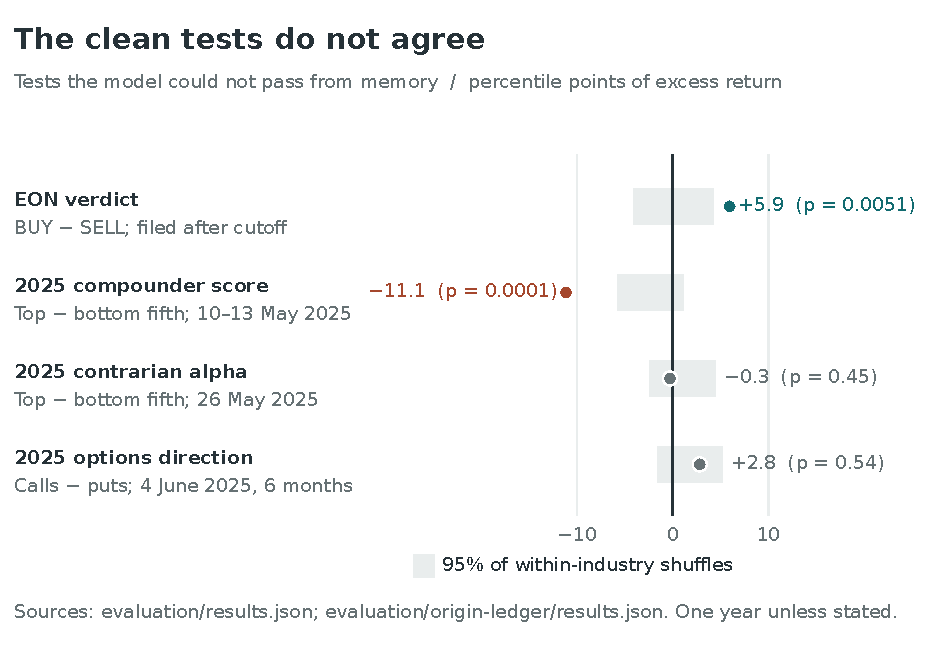
\includegraphics[width=1\linewidth,height=\textheight,keepaspectratio,alt={Four clean tests plotted against their permutation null bands: EON's verdict above its band, the 2025 compounder score far below, the contrarian and options scores inside.}]{figures/09-forward-tests.pdf}
\caption{The clean tests do not agree. Each point is a high-minus-low difference in mean
percentile rank of excess return; grey bands hold 95\% of within-industry shuffles. Only the
EON verdict was read after its outcome window had begun, from filings the model could not have
seen; the three 2025 scores were recorded before any outcome existed. The EON statistic was
chosen after seeing the tails (§8). About 37\% of 2025 ledger companies have no industry label
and share one block. Sources: evaluation/results.json;
evaluation/origin-ledger/results.json.}\label{fig:09-forward-tests}
\end{figure}

These results do not contradict the EON verdicts: across 1,054 companies in both sets, the
verdict and the compounder score are almost unrelated (Spearman 0.05). They are different
judgements. They do share a market: May 2025 to May 2026, a year in which the median stock in
the ledger trailed SPY by more than ten points.

\subsection{9.6 Conviction adds little}\label{conviction-adds-little}

The February report found that high-conviction calls roughly doubled the spread. With better
parsing and the full panel, it does not. At one year, 653 high-conviction BUY and 729
high-conviction SELL readings give 13.3 points, against 11.9 for all readings. Conviction
labels are real but add little information beyond the verdict.

\subsection{9.7 Reading the results together}\label{reading-the-results-together}

Two explanations fit the historical result. The model may have known how those years went. Or
its lenses, which favour strong balance sheets and durable businesses, may have suited 2021 to
2024, when such companies did well. The historical data cannot separate them. They are not
mutually exclusive.

The post-cutoff data add one observation to that argument. The industry tilt, the part most
easily explained by hindsight about sectors, disappears after the cutoff. The within-industry
spread, the part that looks most like reading a filing carefully, mostly stays. That is the
pattern skill would produce. It rests on one vintage, one regime and a statistic chosen after
seeing the tails.

Across every test the model could not have passed from memory, one points up, one points down
and two point nowhere (Figure 9).

\begin{quote}
Before the cutoff, EON's verdicts sorted winners from losers too well to trust. After it, one
verdict still sorts them and another sorted them backwards. A fluent reader is not thereby a
forecaster.
\end{quote}

\FloatBarrier
\section{10. What the work taught me}\label{what-the-work-taught-me}

\subsection{10.1 Fix the question before measuring the answer}\label{fix-the-question-before-measuring-the-answer}

The workflow builder produced better individual analyses than the market-wide batch. It
produced no evidence. Only a fixed schema, applied to everything, made the model's judgement
something that could be counted, compared and tested.

\subsection{10.2 Engineer for the scarcest resource}\label{engineer-for-the-scarcest-resource}

For EON the scarce resource was requests, not compute or storage. That made per-year
checkpoints, leases, resumption and quota-aware waiting the core of the system. It also made
call count a design variable: one call for a wide screener, four for a framework too large for
one schema.

\subsection{10.3 Let the model judge; let code count}\label{let-the-model-judge-let-code-count}

Two lessons point the same way. The February backtest found that the model's categorical
verdict carried more signal than an additive composite of its own sub-scores. The CSPP rewrite
found that the model's arithmetic drifts. Ask the model for judgements on anchored scales, and
do the adding in code, where it can be audited and reweighted.

\subsection{10.4 Date everything the model sees and says}\label{date-everything-the-model-sees-and-says}

The most useful field in the database turned out to be \passthrough{\lstinline!filing\_date!}.
It made entry dates exact and made the cutoff test possible. Every reading should carry the
model's identity and cutoff alongside the filing's date.

\subsection{10.5 An underpowered null is not a negative result}\label{an-underpowered-null-is-not-a-negative-result}

The first run, on prices ending in February 2026, found a post-cutoff six-month spread of +1.0
points, and \ensuremath{-}0.1 within industry. It was tempting to report that the effect vanished. The test
could only have detected about 8 to 10 points. With more filings observed, the same test gives
+4.6. ``Could not detect'' is a different finding from ``absent'', and the minimum detectable
size belongs next to every null.

\subsection{10.6 Look at the tails before trusting a mean}\label{look-at-the-tails-before-trusting-a-mean}

A single stock moved the post-cutoff one-year mean by about 10 points. Returns of small
companies are heavy-tailed, and a mean over a few hundred of them can belong to one. A rank
statistic or a median should sit beside every mean.

\subsection{10.7 Resemblance is not a forecast}\label{resemblance-is-not-a-forecast}

The compounder score measured something real: how closely a company's filings resembled those
of proven compounders. It was a sensible idea and a confident model applied it carefully. For
the year that followed, it pointed the wrong way. A plausible reason, untested here, is that
resemblance to past winners was already priced. The lesson is simpler: a score is a hypothesis
until a ledger says otherwise.

\subsection{10.8 Tell the model the date}\label{tell-the-model-the-date}

A model reasons from its training-time present unless told otherwise. In 2025 it dated its work
a year early and proposed options that had already expired. EON's later workflows stamp run
metadata in code; the date belongs in the prompt too.

\section{11. Scope and remaining questions}\label{scope-and-remaining-questions}

\textbf{The historical result cannot separate memory from judgement.} Every outcome before the
cutoff may be in the model's training data. The anachronism probe rules out careless leakage
only.

\textbf{Every clean test shares one market.} The post-cutoff EON sample and the 2025 ledger
both run through 2025 and 2026. A result that holds in one regime may reverse in the next, as
the compounder score may show.

\textbf{The clean evidence is one vintage.} Nearly all post-cutoff filings were published in
the first quarter of 2025 and held through one market: the tariff shock of April 2025 and the
rally that followed. One regime cannot show that a result generalises.

\textbf{The strongest clean result used a statistic chosen late.} The rank statistic was added
after inspecting the tails. It was applied identically to every sample and has no free
parameters, but it was not pre-registered, and the pre-registered six-month test gave p = 0.11
and 0.048.

\textbf{Industry is a control, not a factor model.} Size, value, profitability and momentum are
not controlled. A lens that prefers strong balance sheets is, partly, a quality factor.
Point-in-time fundamentals would be needed to separate them.

\textbf{The universe is survivors.} Companies were chosen from 2026 listings, and 45 companies
acquired or taken private by September 2026 have no refreshed prices. For the 2025 ledger, 120
of 710 additional tickers returned no prices. The direction of this bias for the spread is not
known.

\textbf{One model, one prompt.} All readings come from Gemini 2.5 Flash and one prompt. Other
models, prompts, or the same model at another temperature may disagree.

\textbf{Prices come from one source.} Yahoo Finance adjusted closes, checked for coverage but
not against a second vendor.

\textbf{Returns are not trades.} No transaction costs, borrow costs, position sizing or
capacity are modelled. The spread is a measure of information, not of profit.

\section{12. Future work}\label{future-work}

\subsection{12.1 Keep the ledger}\label{keep-the-ledger}

The 2025 scripts showed what a ledger is worth: it needs no cutoff argument at all. EON should
keep one deliberately. The fiscal 2025 10-Ks filed in early 2026 are not yet in the database,
because the batch ran before most were filed. Reading them now with the same model and prompt,
and freezing each verdict with its date, would roughly double the clean sample by spring 2027.

\subsection{12.2 Freeze the model}\label{freeze-the-model}

The clean window belongs to one model. Switching to a model with a later cutoff moves the line
and turns part of the clean sample back into memory. The evaluation model should be pinned, and
a new model should start its own ledger. Models are retired, so this has a lifespan; the pinned
version and its cutoff should be recorded with every reading.

\subsection{12.3 Read filings anonymously}\label{read-filings-anonymously}

Remove the company's name, ticker, and identifying product names from a sample of historical
filings and read them again. If the historical spread shrinks under anonymity, memory was doing
part of the work. Glasserman and Lin used this design for news headlines.

\subsection{12.4 Control for known factors}\label{control-for-known-factors}

With point-in-time market capitalisation, valuation and profitability, the spread can be tested
within size and quality groups, or against a factor model. That would say whether the verdicts
know anything a quality screen does not.

\subsection{12.5 Hold the hypothesis workflows to the same standard}\label{hold-the-hypothesis-workflows-to-the-same-standard}

The Moonshot \ensuremath{\times} Excellence and CSPP workflows have produced few readings. Before their scores
are trusted, each needs the same treatment: a fixed protocol, dated readings, and a clean
sample after the cutoff.

\section{13. Related work}\label{related-work}

\textbf{Look-ahead bias in language models.} Sarkar and Vafa show that pretrained language
models leak future information into tasks meant to use only the past, and test for it with
events that should be unpredictable. The anachronism probe here is a simple instance of that
idea. \href{https://papers.ssrn.com/sol3/papers.cfm?abstract_id=4754678}{Sarkar and Vafa,
Lookahead Bias in Pretrained Language Models}. Glasserman and Lin measure look-ahead bias in
GPT sentiment scores for news headlines, and remove company identifiers to reduce it.
\href{https://arxiv.org/abs/2309.17322}{Glasserman and Lin, Assessing Look-Ahead Bias in Stock
Return Predictions Generated by GPT Sentiment Analysis}.

\textbf{Language models and returns.} Lopez-Lira and Tang find that ChatGPT's reading of news
headlines predicts next-day returns, and pay close attention to the model's training window.
\href{https://arxiv.org/abs/2304.07619}{Lopez-Lira and Tang, Can ChatGPT Forecast Stock Price
Movements?}. EON differs in its input (whole annual reports), its horizon (months to years) and
its output (a verdict from three stated philosophies).

\textbf{Reading 10-Ks.} Textual analysis of annual reports has a long history. Loughran and
McDonald built finance-specific word lists for 10-Ks, and Cohen, Malloy and Nguyen found that
changes in 10-K text predict returns. These methods count words; EON asks a model for a
judgement. Both face the same question of what the text knows that prices do not.
\href{https://doi.org/10.1111/j.1540-6261.2010.01625.x}{Loughran and McDonald, When Is a
Liability Not a Liability?}; \href{https://doi.org/10.1111/jofi.12885}{Cohen, Malloy and
Nguyen, Lazy Prices}.

\textbf{Multiple testing in finance.} Harvey, Liu and Zhu show how many published return
predictors fail once the number of tests is counted. That argument is why the primary tests
here were fixed first and later additions are labelled.
\href{https://doi.org/10.1093/rfs/hhv059}{Harvey, Liu and Zhu, \ldots{} and the Cross-Section
of Expected Returns}.

\section{14. Conclusion}\label{conclusion}

I set out to build a reader that gives every annual report the same careful attention. It began
in May 2025 as scripts studying excellent companies. The workflow builder showed which
questions were worth asking. Fixing one question and asking it of every filing turned the model
into an instrument. The quota set the pace, and 6,653 readings later there was something to
measure.

The first measurement was too good. It tested the model on years it may already have known.
Rebuilt around the model's knowledge cutoff, the test tells a quieter story. Before the cutoff,
the verdicts separate winners from losers by 13 points a year, and part of that is a bet on
industries. After it, the industry bet is gone, and a smaller within-industry spread remains.
And the scores written down in 2025, before anyone knew the answers, include one that pointed
the wrong way.

That is where the evidence stands today. It will not stay there: every filing season adds
readings the model cannot have memorised. The newspaper the model read ends in January 2025.
Everything after that has to be read the ordinary way, one day at a time.

\FloatBarrier
\section{Appendix A: reproduction}\label{appendix-a-reproduction}

\subsection{Artefacts}\label{artefacts}

{\def\LTcaptype{table} % do not increment counter
\par\addvspace{8pt}\noindent\begin{minipage}{\linewidth}\small
\begin{tabular}{@{}
  >{\raggedright\arraybackslash}p{(\linewidth - 2\tabcolsep) * \real{0.5500}}
  >{\raggedright\arraybackslash}p{(\linewidth - 2\tabcolsep) * \real{0.4500}}@{}}
\toprule\noalign{}
\begin{minipage}[b]{\linewidth}\raggedright\bfseries
Path
\end{minipage} & \begin{minipage}[b]{\linewidth}\raggedright\bfseries
Contents
\end{minipage} \\
\midrule\noalign{}


\passthrough{\lstinline!eon/ai/prompts/perspectives.py!} & The three-lens prompt \\
\passthrough{\lstinline!eon/analysis/perspectives/analyzer.py!} & Filing text to structured
reading \\
\passthrough{\lstinline!eon/ai/providers/gemini.py!} & Model calls, schema validation,
retries \\
\passthrough{\lstinline!eon/ui/services/batch\_queue.py!} & Multi-day batches, leases,
resumption \\
\passthrough{\lstinline!custom\_workflows/cspp\_v26\_analyzer.py!} & Four-call split, totals in
code \\
\passthrough{\lstinline!custom\_workflows/moonshot\_excellence\_finder.py!} & One-call
screener, anchored scales \\
\passthrough{\lstinline!experimental/backtester/BACKTEST\_REPORT.md!} & The February report
(§7.1) \\
\passthrough{\lstinline!docs/whitepaper/evaluation-config.yaml!} & The protocol and its
amendments \\
\passthrough{\lstinline!docs/whitepaper/origin-ledger-config.yaml!} & The 2025 ledger
protocol \\
\passthrough{\lstinline!stock\_stuff\_06042025/10K\_automator/!} & The 2025 origin scripts and
outputs (read-only) \\
\bottomrule\noalign{}
\end{tabular}
\end{minipage}\par\addvspace{8pt}
}

\subsection{Rebuilding the evaluation, figures and paper}\label{rebuilding-the-evaluation-figures-and-paper}

\par\noindent\begin{minipage}{\linewidth}

From the eon root. The database is opened read-only; outputs go only to
\passthrough{\lstinline!docs/whitepaper/!}. The price refresh needs network access and
yfinance; every other step runs offline. Evaluation and figures need NumPy, pandas, SciPy,
Matplotlib and PyYAML.

\par\noindent\begin{minipage}{\linewidth}
\begin{lstlisting}[language=sh]
python docs/whitepaper/refresh_prices.py        # optional: fetch new prices
python docs/whitepaper/evaluate_backtest.py     # about 30 seconds
python docs/whitepaper/refresh_prices.py --origin   # optional: 2025 ledger tickers
python docs/whitepaper/evaluate_origin_ledger.py
python docs/whitepaper/prepare_figure_data.py
python docs/whitepaper/render_figures.py
python docs/whitepaper/build_paper.py           # needs Pandoc 3.x
\end{lstlisting}
\end{minipage}\par

\end{minipage}\par

A refresh moves \passthrough{\lstinline!price\_end!} only if the config is changed. Every
script writes a \passthrough{\lstinline!run.json!} with its configuration and the hashes of its
inputs and outputs. The refreshed price file is local and not committed; its hash is recorded.

\clearpage
\section{Appendix B: glossary}\label{appendix-b-glossary}

\textbf{Reading.} One model call on one 10-K, stored as 35 validated fields.

\textbf{Vintage.} All readings with the same fiscal-year label.

\textbf{Verdict.} The first word of the final verdict: STRONG BUY, BUY, HOLD, SELL or STRONG
SELL. BUY and STRONG BUY form the long leg; SELL and STRONG SELL the short.

\textbf{Excess return.} A stock's return minus SPY's over the same window, from the first
trading day after the filing.

\textbf{Spread.} Mean excess return of the long leg minus that of the short leg, in percentage
points.

\textbf{Rank spread.} The same difference, using each reading's percentile rank of excess
return within its vintage. One extreme return cannot decide it.

\textbf{Knowledge cutoff.} The date after which a model's training data is said to end. For
Gemini 2.5 Flash, January 2025; this paper uses 31 January 2025.

\textbf{Industry tilt.} The mean of the within-industry permutation null: the spread expected
from the model's choice of industries alone.

\textbf{Minimum detectable spread.} About 2.8 times the permutation null's standard deviation:
the spread a test would detect with 80\% power at p \textless{} 0.05.

\textbf{Anachronism.} A reading that mentions something that did not exist when its filing was
published.

\clearpage
\section{Appendix C: figures at a glance}\label{appendix-c-figures-at-a-glance}

\par\noindent\begin{minipage}{\linewidth}
\begin{lstlisting}
ORIGIN, MAY-JUNE 2025     11,741 filing readings, 2,175 companies
                          scores recorded before their outcomes
READINGS                  6,653 company-years, 1,358 companies
MODEL                     Gemini 2.5 Flash, cutoff January 2025
SCHEMA                    35 fields: 3 lenses x 11, synthesis, verdict
MARKET BATCH              6,568 readings in 13 days, 8-21 Feb 2026
QUOTA                     25 keys x 20 requests = 500 readings a day

VERDICT MIX               HOLD 50.8%  BUY 27.5%  SELL 16.5%
                          STRONG BUY 3.8%  STRONG SELL 1.4%

FEBRUARY REPORT           2Y spread +14.1 pts (reported; pre-cutoff)

BEFORE CUTOFF, 1Y         +13.1 pts  (1,099 BUY / 657 SELL)  p = 0.0001
  rank spread             11.5: 4.8 industry tilt, 6.6 within industry
AFTER CUTOFF, 6M          +4.6 pts   (416 / 275)  p = 0.11; 0.048 by industry
AFTER CUTOFF, 1Y mean     +14.9 pts  (339 / 201)  +/-23; p = 0.22
  one stock (BW)          adds about 10 pts to the BUY mean
AFTER CUTOFF, 1Y rank     5.9: 0.1 industry tilt, 5.9 within  p = 0.0051
                          (rank statistic added after seeing the tails)

2025 LEDGER, 1Y           compounder: Spearman -0.14  p = 0.0001
                          contrarian alpha: +0.01  p = 0.71
                          options direction (6M): +2.8  p = 0.54
ANACHRONISM PROBE         0 early mentions; IRA in 300 readings
HIGH CONVICTION, 1Y       +13.3 pts vs +11.9 for all readings

NOT YET MEASURED          2Y after cutoff; anonymised reading; a second regime;
                          factor controls; a second clean vintage
\end{lstlisting}
\end{minipage}\par

\emph{Prepared from the EON repository, its analysis database, and a price refresh of 29
September 2026. Figures are drawn from a checked-in evidence snapshot with source hashes.
Negative and inconclusive results are retained. This paper is research, not investment advice.
See figures.md for figure provenance and revision-notes.md for what needs the author's
confirmation.}

\end{document}
